% ============================================
% Chapitre 3 : Instances EC2
% ============================================
\chapter{Architecture des Instances EC2}
\label{chap:instances}

\section{Vue d'Ensemble des Instances}

Trois instances EC2 ont été déployées pour ce projet, chacune ayant un rôle spécifique dans l'infrastructure de monitoring.

\begin{table}[H]
\centering
\caption{Récapitulatif des instances EC2}
\label{tab:instances-summary}
\begin{tabular}{|l|l|l|l|}
\hline
\textbf{Instance} & \textbf{Type} & \textbf{OS} & \textbf{Rôle} \\
\hline
ELBadry-Zabbix-Server & t3.large & Ubuntu 22.04 & Serveur Zabbix (Docker) \\
\hline
ELBadry-Client-Linux & t3.medium & Ubuntu 22.04 & Client supervisé \\
\hline
ELBadry-Client-Windows & t3.large & Windows Server 2022 & Client supervisé \\
\hline
\end{tabular}
\end{table}

\begin{figure}[H]
\centering
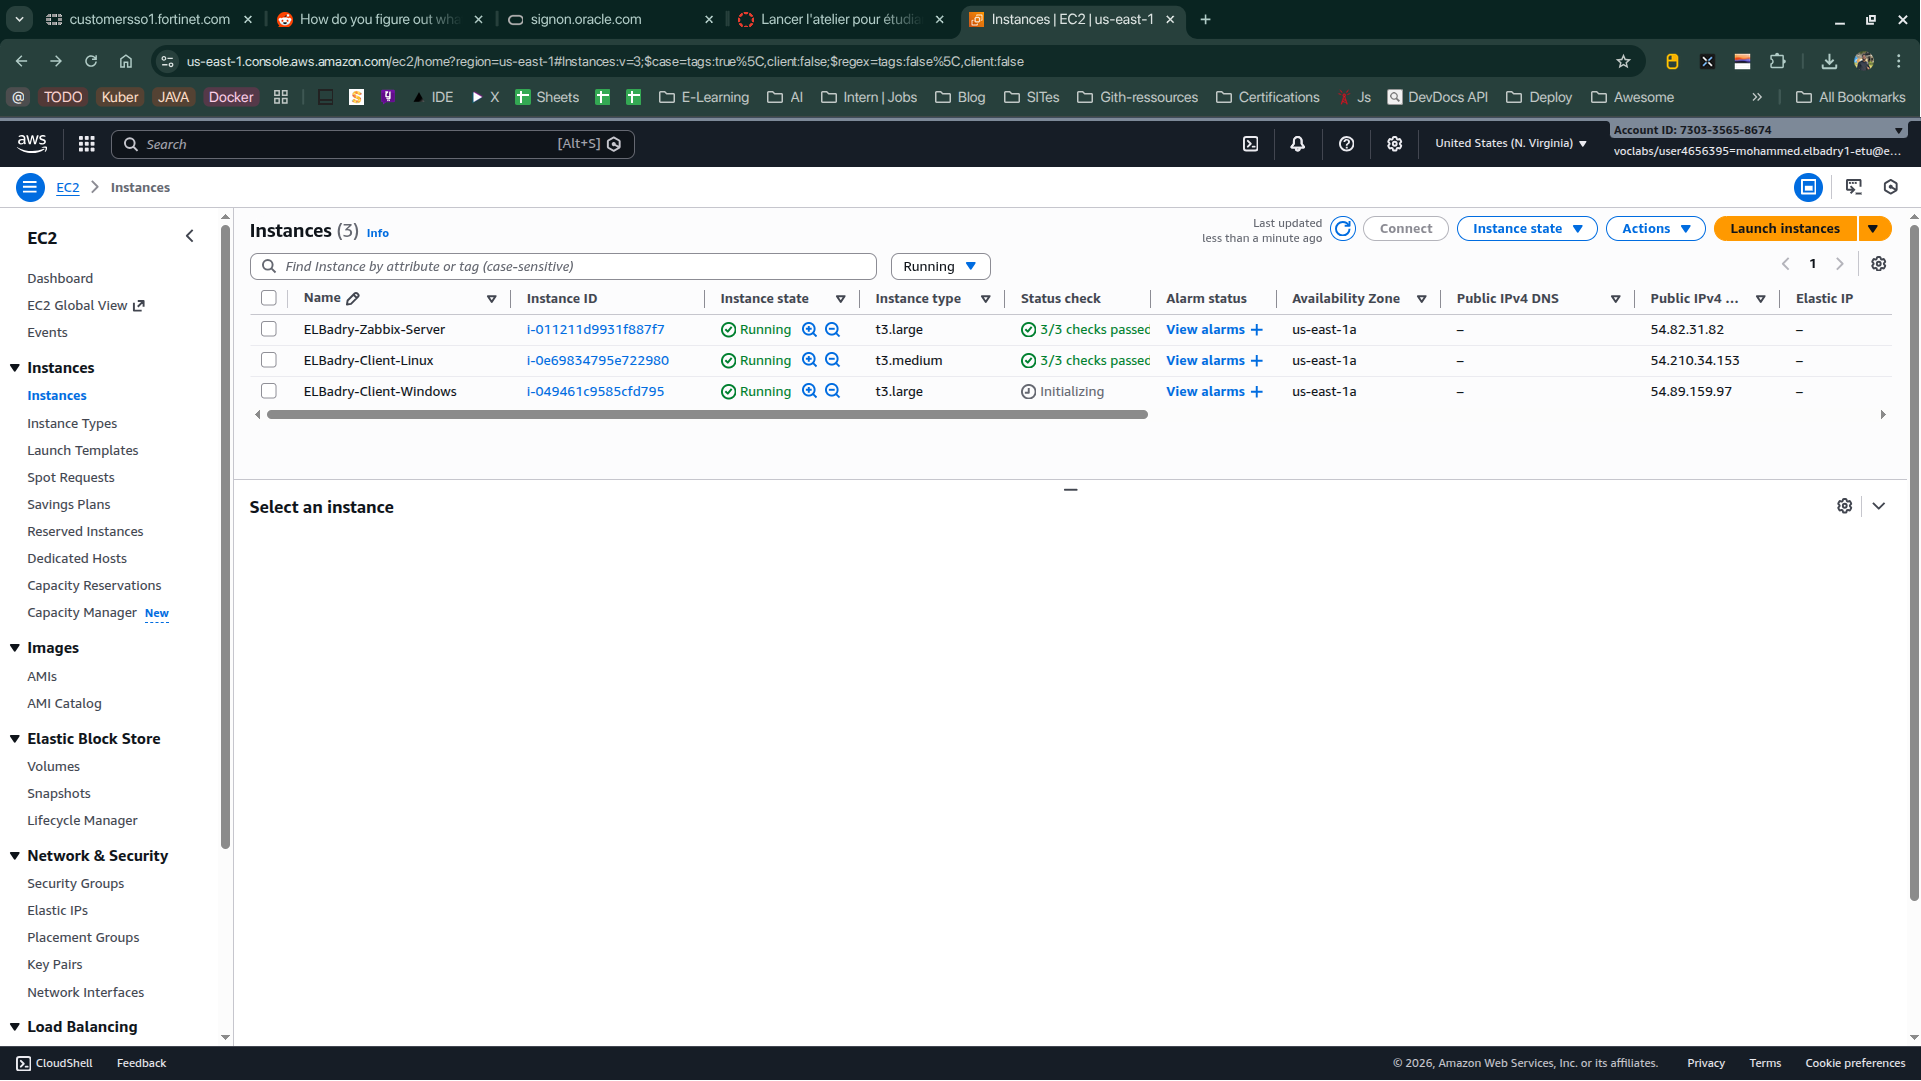
\includegraphics[width=0.95\textwidth]{images/03-instances-list-status.png}
\caption{Liste des instances EC2 en état Running}
\label{fig:instances-list}
\end{figure}

\section{Serveur Zabbix}

\subsection{Spécifications}

Le serveur Zabbix est le cœur de l'infrastructure de monitoring :

\begin{table}[H]
\centering
\caption{Configuration du serveur Zabbix}
\label{tab:zabbix-server-config}
\begin{tabular}{|l|l|}
\hline
\textbf{Paramètre} & \textbf{Valeur} \\
\hline
Nom & ELBadry-Zabbix-Server \\
\hline
Type d'instance & t3.large (2 vCPU, 8 Go RAM) \\
\hline
AMI & Ubuntu Server 22.04 LTS \\
\hline
Stockage & 30 Go gp3 \\
\hline
IP Privée & 10.0.1.x \\
\hline
Security Group & ELBadry-Zabbix-Server-SG \\
\hline
\end{tabular}
\end{table}

\begin{figure}[H]
\centering
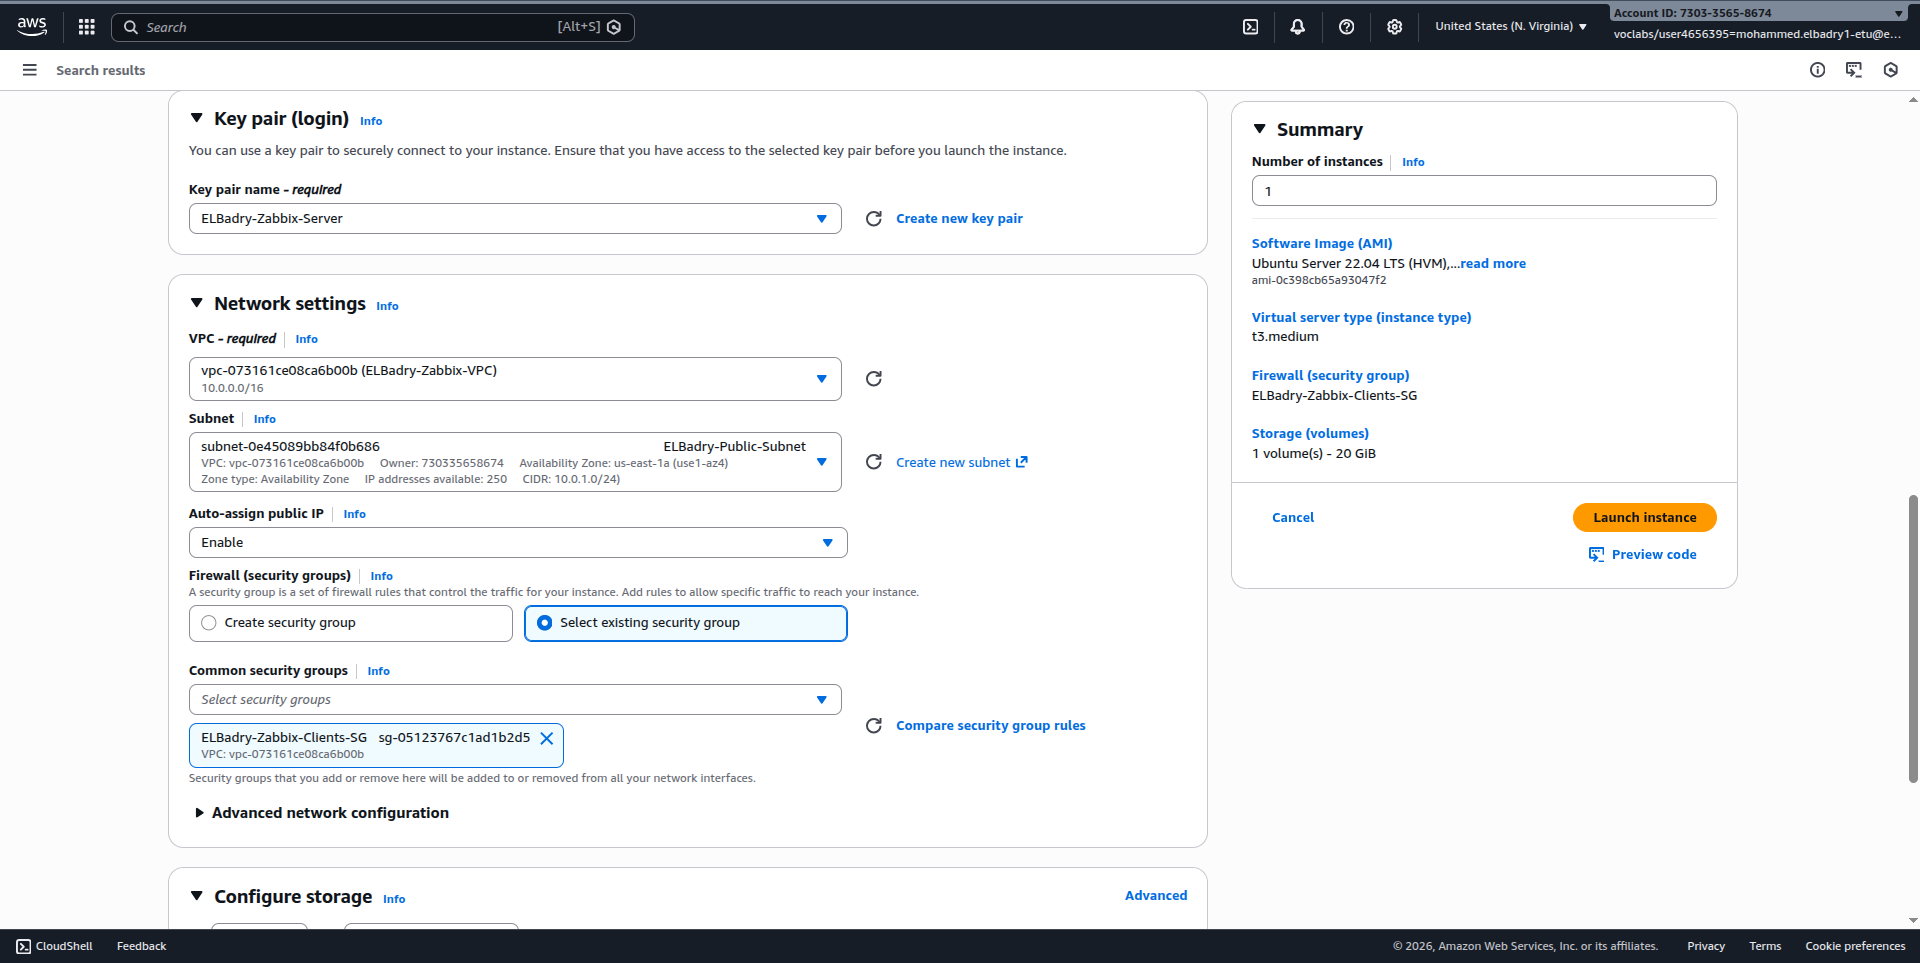
\includegraphics[width=0.95\textwidth]{images/05-instance-zabbix-server-details.png}
\caption{Détails de l'instance Zabbix Server}
\label{fig:zabbix-server-details}
\end{figure}

\subsection{Justification du Choix t3.large}

Le type t3.large a été choisi pour le serveur Zabbix car :
\begin{itemize}
    \item \textbf{8 Go de RAM} : Suffisant pour Docker, MySQL et Zabbix Server
    \item \textbf{2 vCPU} : Permet de gérer plusieurs conteneurs simultanément
    \item \textbf{Performances en rafale} : Adapté aux pics de charge
    \item \textbf{Compatible Learner Lab} : Type d'instance autorisé
\end{itemize}

\section{Client Linux}

\subsection{Spécifications}

\begin{table}[H]
\centering
\caption{Configuration du client Linux}
\label{tab:client-linux-config}
\begin{tabular}{|l|l|}
\hline
\textbf{Paramètre} & \textbf{Valeur} \\
\hline
Nom & ELBadry-Client-Linux \\
\hline
Type d'instance & t3.medium (2 vCPU, 4 Go RAM) \\
\hline
AMI & Ubuntu Server 22.04 LTS \\
\hline
Stockage & 20 Go gp3 \\
\hline
IP Privée & 10.0.1.x \\
\hline
Security Group & ELBadry-Zabbix-Clients-SG \\
\hline
\end{tabular}
\end{table}

\begin{figure}[H]
\centering
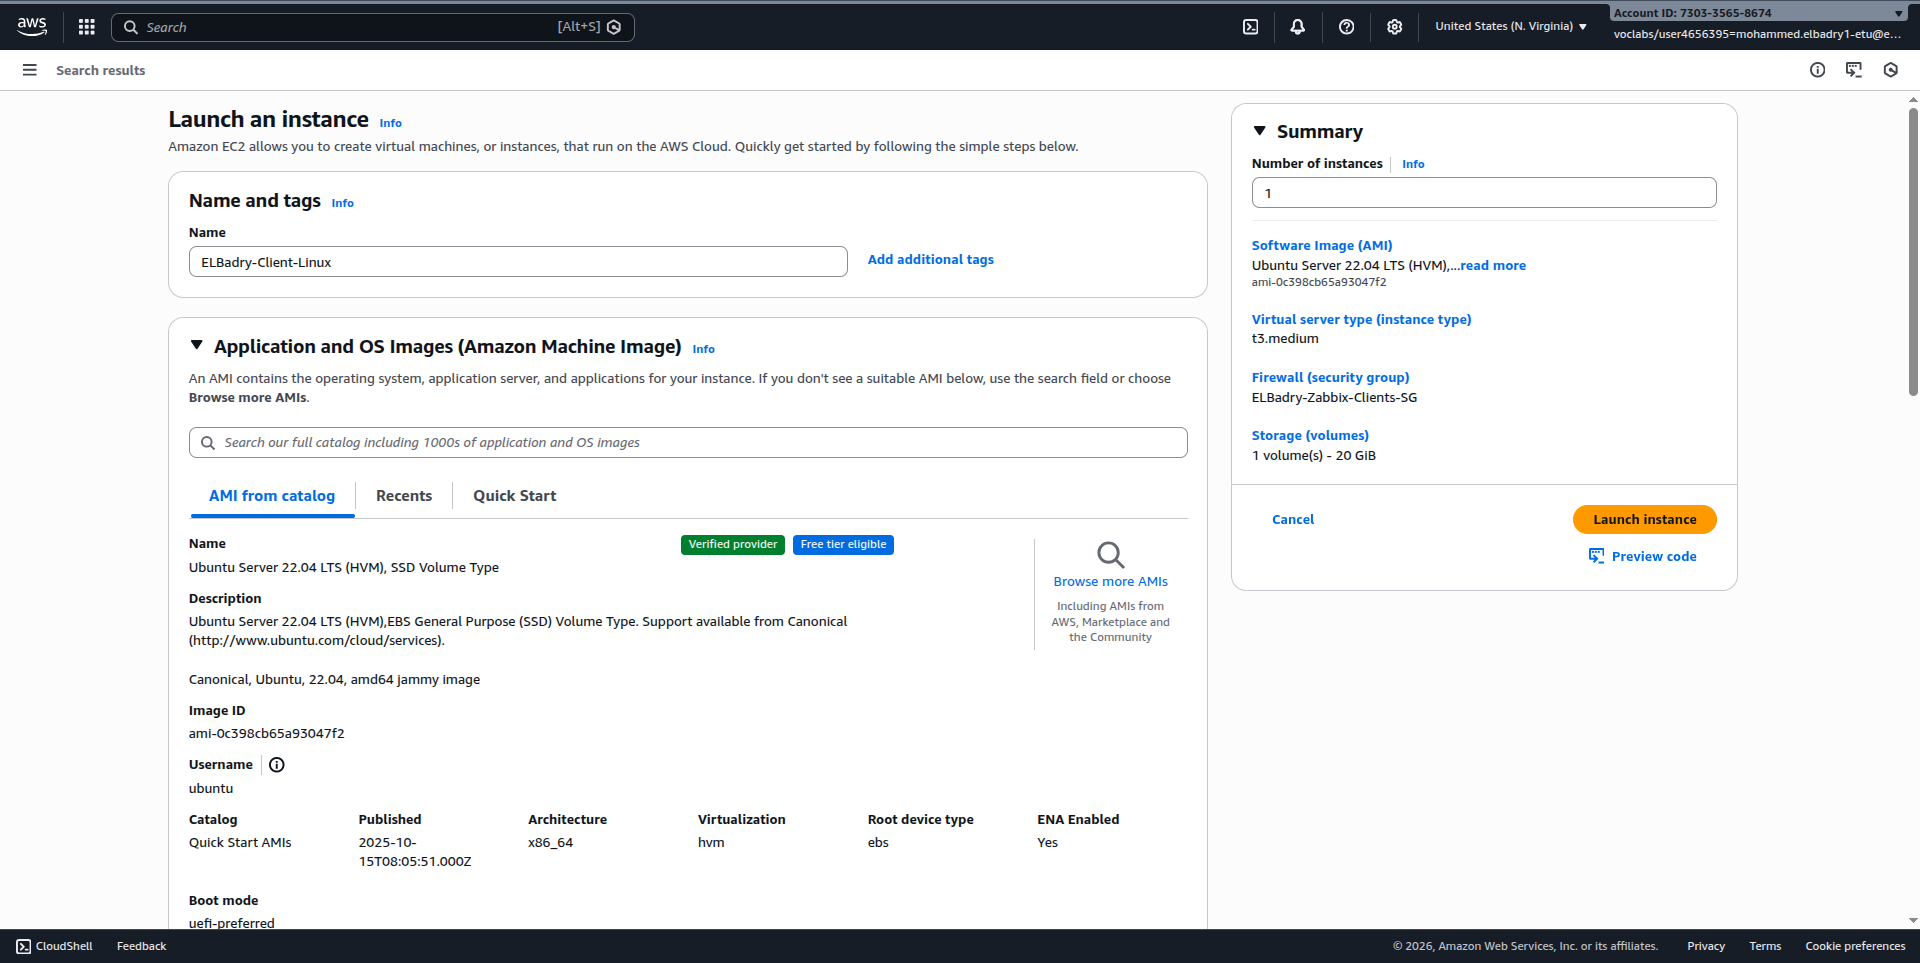
\includegraphics[width=0.95\textwidth]{images/10-instance-client-linux-details.png}
\caption{Détails de l'instance Client Linux}
\label{fig:client-linux-details}
\end{figure}

\section{Client Windows}

\subsection{Spécifications}

\begin{table}[H]
\centering
\caption{Configuration du client Windows}
\label{tab:client-windows-config}
\begin{tabular}{|l|l|}
\hline
\textbf{Paramètre} & \textbf{Valeur} \\
\hline
Nom & ELBadry-Client-Windows \\
\hline
Type d'instance & t3.large (2 vCPU, 8 Go RAM) \\
\hline
AMI & Microsoft Windows Server 2022 Base \\
\hline
Stockage & 30 Go gp3 \\
\hline
IP Privée & 10.0.1.x \\
\hline
Security Group & ELBadry-Zabbix-Clients-SG \\
\hline
\end{tabular}
\end{table}

\begin{figure}[H]
\centering
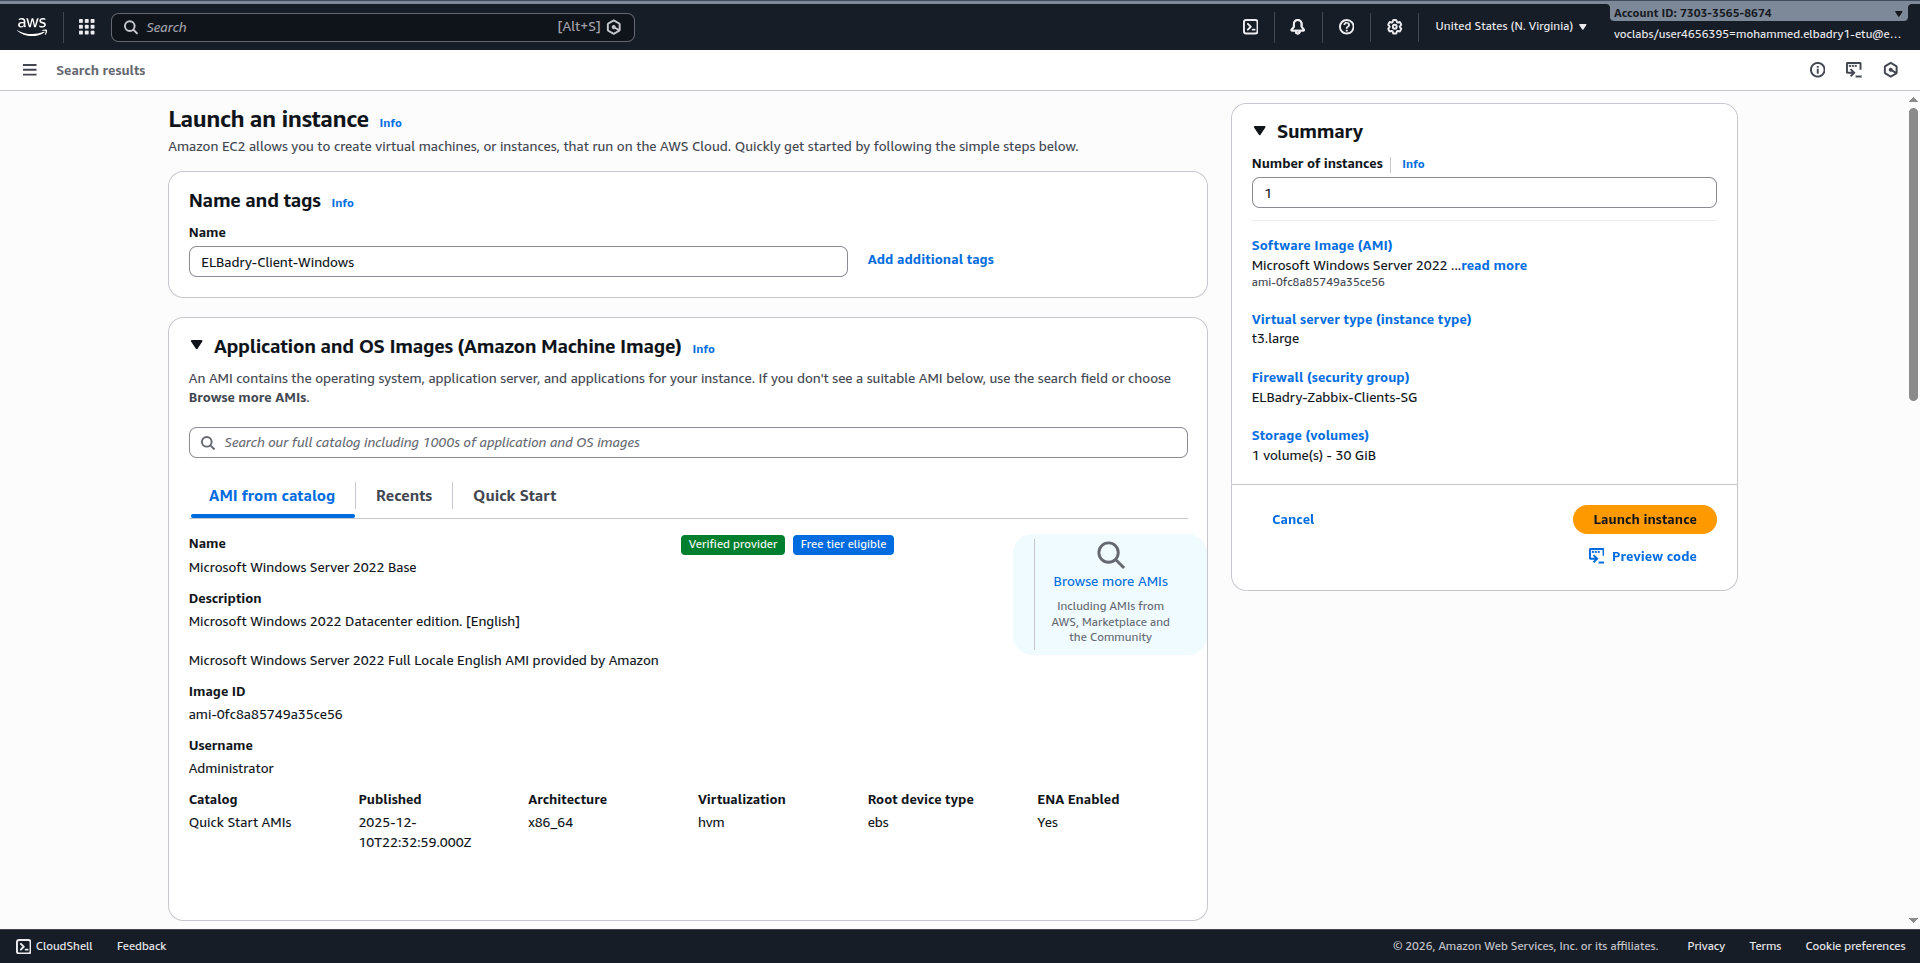
\includegraphics[width=0.95\textwidth]{images/11-instance-client-windows-details.png}
\caption{Détails de l'instance Client Windows}
\label{fig:client-windows-details}
\end{figure}

\subsection{Récupération du Mot de Passe Windows}

Pour accéder au client Windows via RDP, il est nécessaire de récupérer le mot de passe administrateur :

\begin{enumerate}
    \item Sélectionner l'instance Windows
    \item Actions → Security → Get Windows Password
    \item Charger la clé privée (.pem)
    \item Déchiffrer le mot de passe
\end{enumerate}

\begin{figure}[H]
\centering
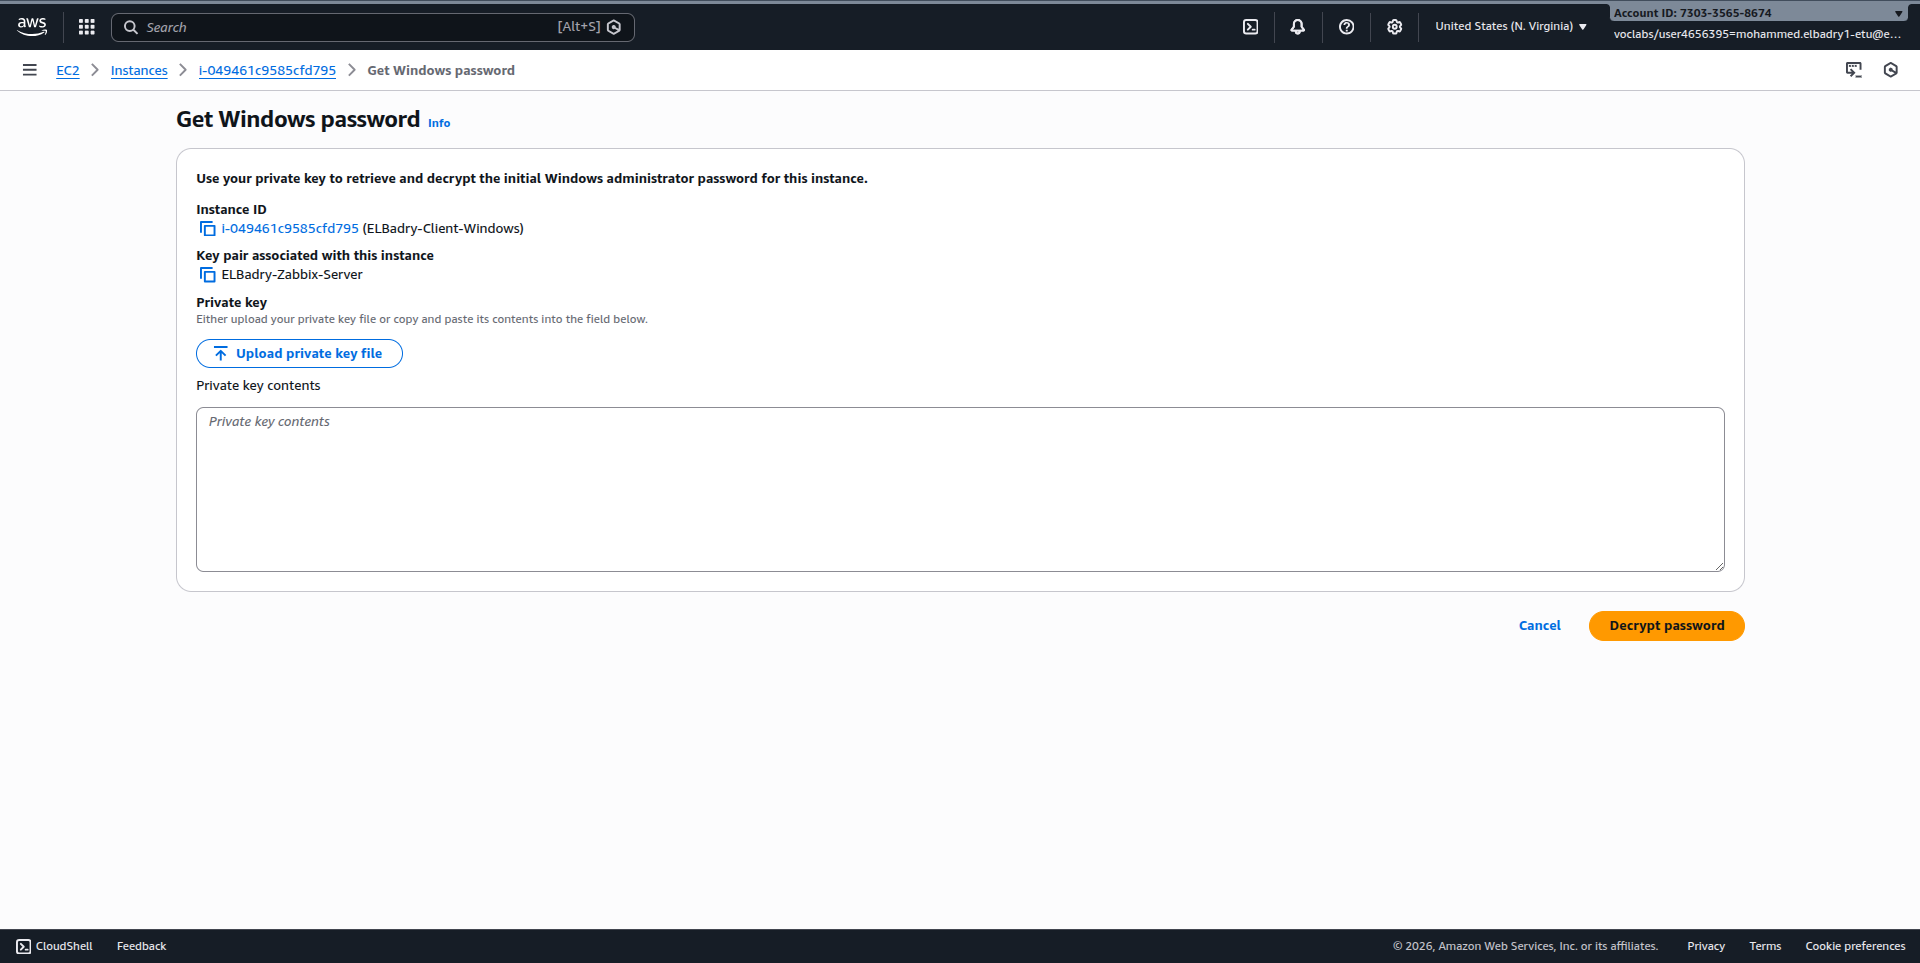
\includegraphics[width=0.85\textwidth]{images/12-windows-get-password.png}
\caption{Récupération du mot de passe Windows}
\label{fig:windows-password}
\end{figure}

\section{Connexion aux Instances}

\subsection{Connexion SSH au Serveur Zabbix}

\begin{lstlisting}[language=bash, caption=Connexion SSH au serveur Zabbix]
ssh -i "votre-cle.pem" ubuntu@<IP-PUBLIQUE-ZABBIX>
\end{lstlisting}

\begin{figure}[H]
\centering
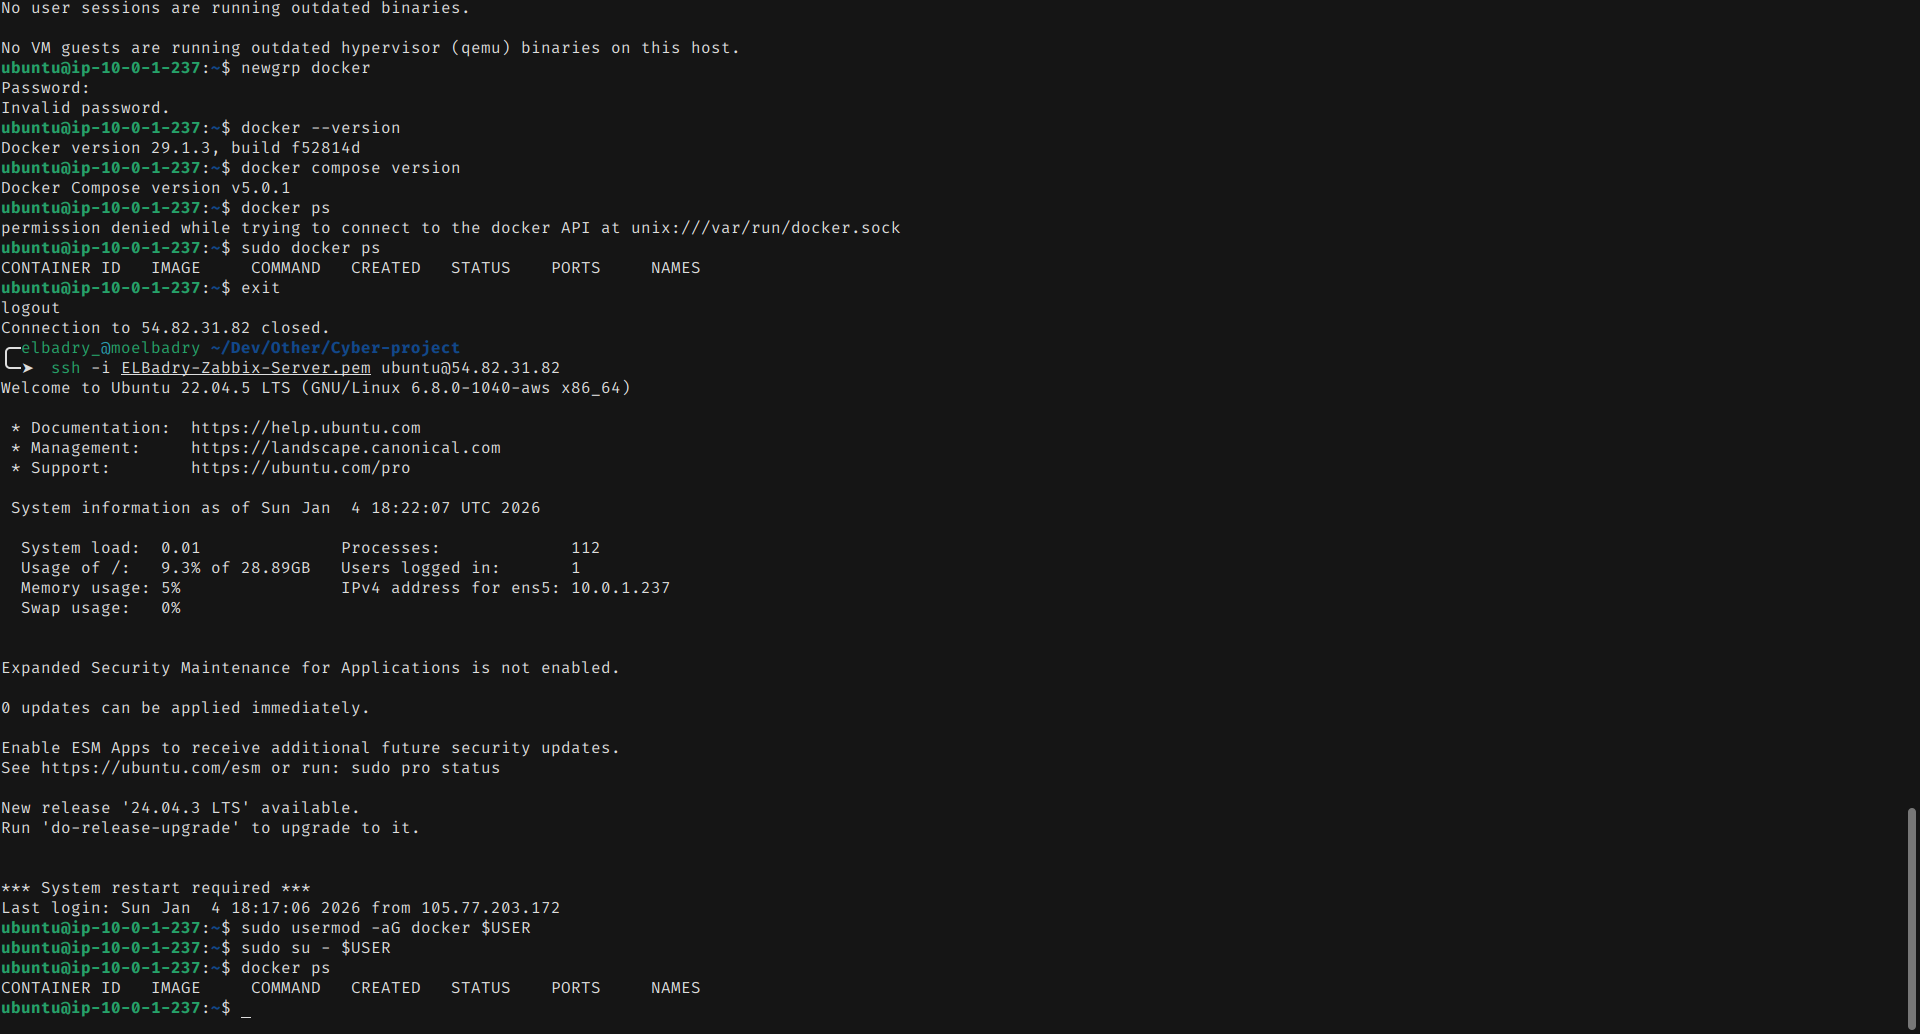
\includegraphics[width=0.95\textwidth]{images/13-ssh-connection-server.png}
\caption{Connexion SSH réussie au serveur Zabbix}
\label{fig:ssh-connection}
\end{figure}

\subsection{Connexion RDP au Client Windows}

\begin{enumerate}
    \item Ouvrir le client Bureau à distance (mstsc)
    \item Entrer l'IP publique de l'instance Windows
    \item Utiliser le nom d'utilisateur : \texttt{Administrator}
    \item Entrer le mot de passe déchiffré
\end{enumerate}

\begin{figure}[H]
\centering
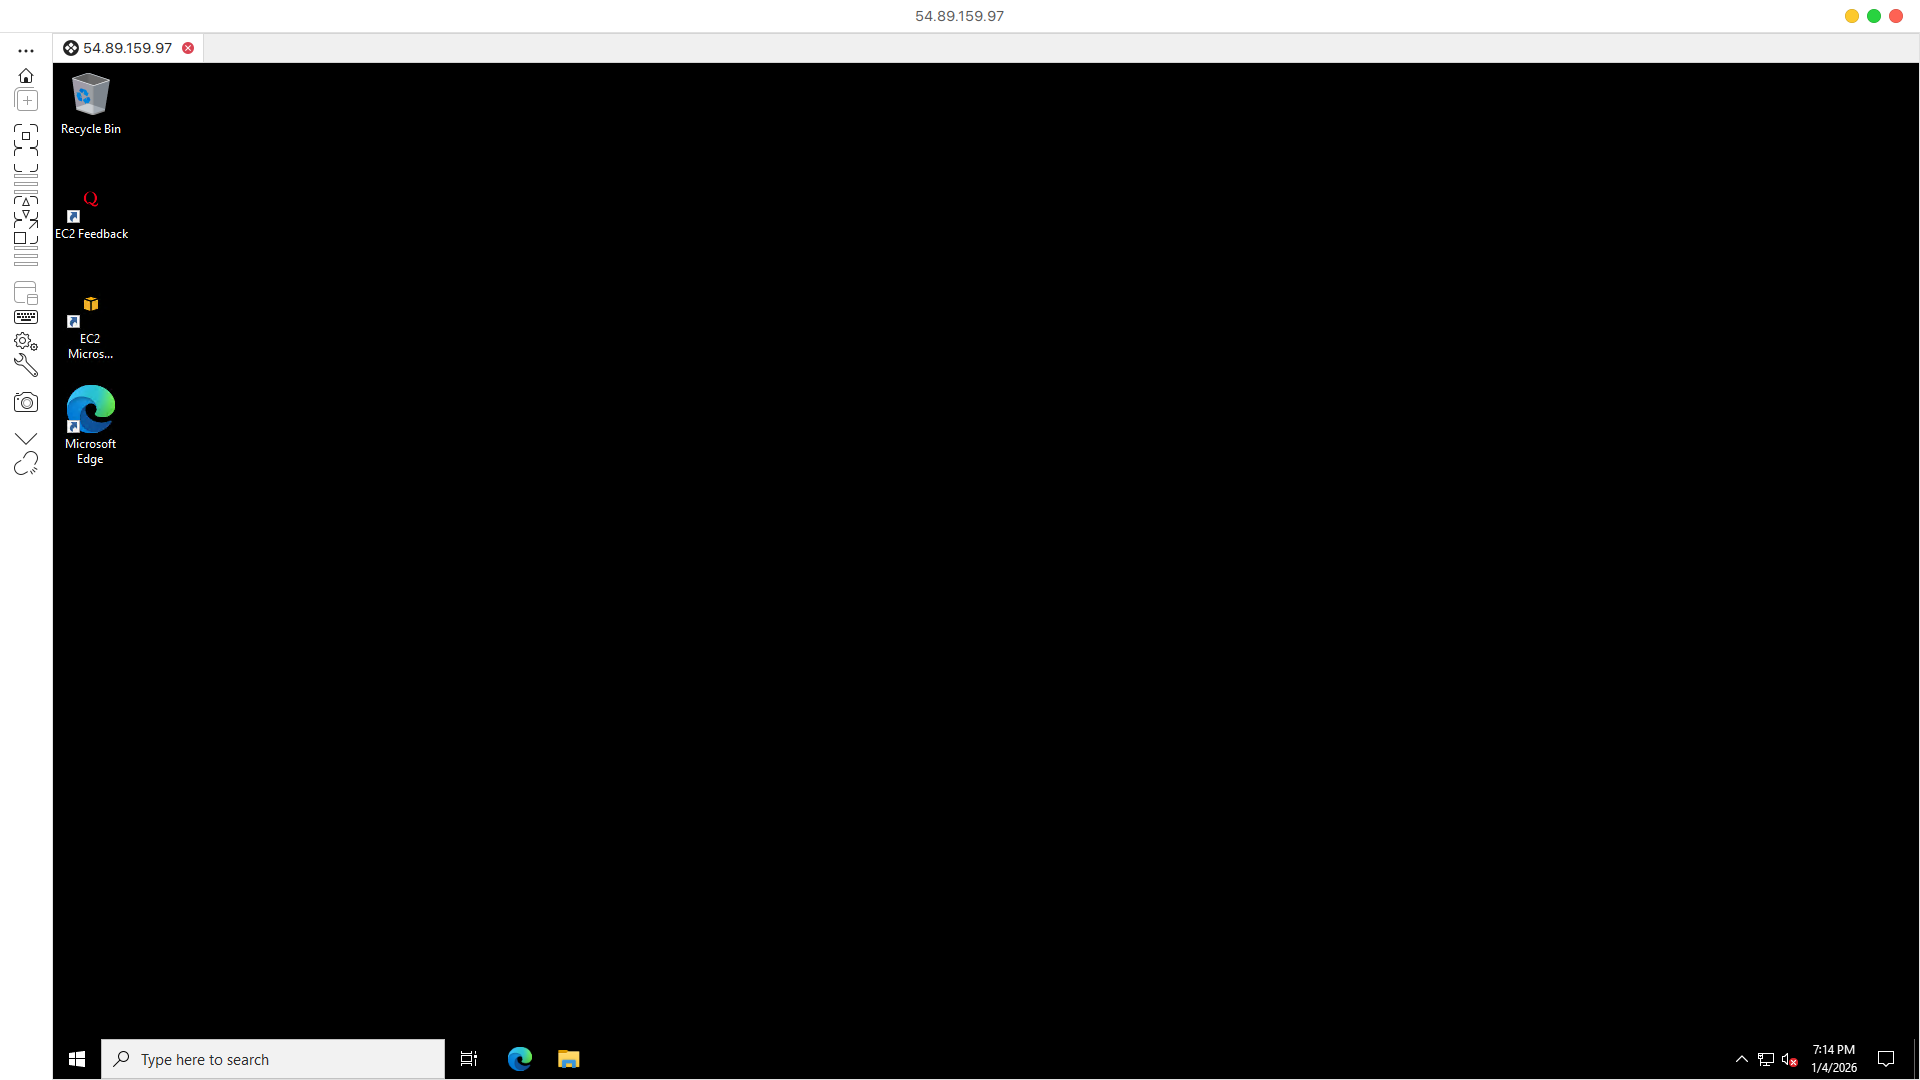
\includegraphics[width=0.85\textwidth]{images/21-windows-rdp-connection.png}
\caption{Connexion RDP au client Windows}
\label{fig:rdp-connection}
\end{figure}

\section{Tableau Récapitulatif}

\begin{table}[H]
\centering
\caption{Récapitulatif complet des instances}
\label{tab:instances-full}
\begin{tabular}{|l|c|c|c|}
\hline
\textbf{Propriété} & \textbf{Zabbix Server} & \textbf{Client Linux} & \textbf{Client Windows} \\
\hline
Type & t3.large & t3.medium & t3.large \\
\hline
vCPU & 2 & 2 & 2 \\
\hline
RAM & 8 Go & 4 Go & 8 Go \\
\hline
OS & Ubuntu 22.04 & Ubuntu 22.04 & Windows Server 2022 \\
\hline
Stockage & 30 Go & 20 Go & 30 Go \\
\hline
Accès & SSH (22) & SSH (22) & RDP (3389) \\
\hline
\end{tabular}
\end{table}
